%%%%%%%%%%%%%%%%%%%%%%%%%%%%%%%%%%%%%%%%%%%%%%%%%%%%%%%%%%%%%%%%%%%%%%
% LaTeX Template: Beamer arrows
%
% Source: http://www.texample.net/
% Feel free to distribute this template, but please keep the
% referal to TeXample.net.
% Date: Nov 2006
% 
%%%%%%%%%%%%%%%%%%%%%%%%%%%%%%%%%%%%%%%%%%%%%%%%%%%%%%%%%%%%%%%%%%%%%%
% How to use writeLaTeX: 
%
% You edit the source code here on the left, and the preview on the
% right shows you the result within a few seconds.
%
% Bookmark this page and share the URL with your co-authors. They can
% edit at the same time!
%
% You can upload figures, bibliographies, custom classes and
% styles using the files menu.
%
% If you're new to LaTeX, the wikibook is a great place to start:
% http://en.wikibooks.org/wiki/LaTeX
%
%%%%%%%%%%%%%%%%%%%%%%%%%%%%%%%%%%%%%%%%%%%%%%%%%%%%%%%%%%%%%%%%%%%%%%

\documentclass[9pt]{beamer} %
\usetheme{CambridgeUS}
%\usetheme{Copenhagen}
\usepackage[latin1]{inputenc}
\usepackage{pifont}
\usefonttheme{professionalfonts}
\usepackage{times}
\usepackage{bbm}
\usepackage{tikz}
\usepackage{amsmath}
\usepackage{verbatim}
\usepackage{graphicx}
\usepackage{ragged2e}
\usetikzlibrary{arrows,shapes}
\usepackage{natbib}
\setbeamertemplate{navigation symbols}{}
\justifying
\defcitealias{becker2019deep}{Deep optimal stopping}
\newcommand{\gooditem}[1]{\setbeamercolor{item}{fg=darkred}\item #1} 

\author{Claudia Viaro}
\title[Optimal stopping \& switching]{Optimal stopping \& switching by approximating the indicator function with neural networks}

\begin{document}

\maketitle




% For every picture that defines or uses external nodes, you'll have to
% apply the 'remember picture' style. To avoid some typing, we'll apply
% the style to all pictures.
\tikzstyle{every picture}+=[remember picture]

% By default all math in TikZ nodes are set in inline mode. Change this to
% displaystyle so that we don't get small fractions.
\everymath{\displaystyle}
\begin{frame}{Outline}
    \tableofcontents
\end{frame}
% Presentation structure
\section{Optimal stopping problems}
\section{Approximation methods}
\section{Approximating the indicator function}
    \subsection{Define stopping decisions}
    \subsection{Approximating stopping decisions}
    \subsection{}
\section{Optimal switching problems}
\section*{References}
\begin{frame}
% to enforce entries in the table of contents
\end{frame}

\AtBeginSection[]
{
    \begin{frame}
        \frametitle{Table of Contents}
        \tableofcontents[currentsection]
    \end{frame}
}


\begin{frame}
\frametitle{Optimal stopping problems}

\begin{block}{Definition}
Let $(\Omega, \mathcal{F},(\mathcal{F}_n)_{n\geq 0},\mathbb{P})$ be a filtered probability space and $X = (X_n)_{n\geq 0}^N $ an $\mathbb{R}^d$-valued discrete-time stochastic process on it, describing the price of $d$ stock prices under the risk-neutral measure $\mathbb{P}$.

\medskip
For a finite time horizon $T \in \mathbb{N}$, denote by $\mathfrak{M}^T$ the class of all stopping times $\tau$ of the filtration $(\mathcal{F}_n)_{n\geq 0}$: the random variables $0 \leq \tau \leq N$ are finite a.s. and $\{\tau = n \} \in \mathcal{F}_n$ for all $n \in \{ 0, 1, \ldots, N\}$.

\medskip
The optimal stopping problem
\begin{equation}\label{eq1}
    V=\sup_{\tau \in \mathcal{T}} \mathbb{E} g(\tau, X_{\tau})
\end{equation}
consists in finding the quantity $V$ and a stopping time $\tau^{\ast} \in \mathfrak{M}^T$ at which the supremum is attained (if it exists), where $g: [0,N] \times \mathbb{R}^d \rightarrow \mathbb{R}$ is a discounted payoff function.
\end{block}
\end{frame}

\begin{frame}{An exact solution}
   Optimal stopping problems can be solved exactly:
   \begin{itemize}
       \gooditem $V^{\ast}$ is the Snell envelope
       \begin{equation}\label{eq2}
       \begin{split}
           &U_N := g(X_N),\\
           &U_n := \max (g(X_n), \mathbb{E}[\alpha U_{n+1} | X_n]),
       \end{split}   
       \end{equation}
       where $\alpha$ is a discount factor. Equivalently, $U_n$ can be expressed as the optimal stopping problem:
       \begin{equation}\label{eq3}
           U_n = \sup_{\tau \in \Tau_n} \mathbf{E}[\alpha^{\tau - n}g(X_{\tau}| X_n]
       \end{equation}
       where $\tau_n$ is the set of all stopping times $\tau \leq n$
       \gooditem $\tau^{\ast}$ is the first time the immediate reward dominates the continuation value
       \begin{equation}\label{eq4}
       \begin{split}
       &\tau_N := N,\\
       &\tau_n := \begin{cases} 
       n, & \mbox{if } g(X_n) \geq \mathbb{E}[\alpha U_{n+1}| X_n] \\ 
       \tau_{n+1}, & \mbox{otherwise.}  \end{cases}
       \end{split}
       \end{equation}
   \end{itemize}
\end{frame}

\begin{frame}{Approximation methods with NN}
$\rightarrow$ numerical methods suffer from the curse of dimensionality ($d$ assets)

\medskip
A more recent line of research use backward recursion and stochastic gradient based methods to tackle high dimensional stopping problems.
\medskip

Consider $m$ realizations from a $d$-dimensional Markovian stochastic process $X$ under $\mathbb{Q}$, where the $i$-th realization is $x_0, x_1^i, \ldots, x_N^i$, with fixed spot price $x_0$. For each $m$ the price, under stopping strategy \ref{eq1}, is:


\begin{equation}\label{eq5}
       \begin{split}
           &p_N^i := g(x^i_N),\\
           &p_n^i := \begin{cases} 
       g(x^i_n), & \mbox{if } g(x^i_n) \geq c_n(x^i_n), \\ 
          \alpha p^i_{n+1}, & \mbox{otherwise.}  \end{cases}
       \end{split}   
       \end{equation}
where $c_n(x_n^i)$ is the continuation value       
\end{frame}
 
\begin{frame}{}
Stochastic gradient based methods are used to optimize the parameters $\theta_n$ of a neural network that approximates either: 
\begin{itemize}
\gooditem the continuation value \citep{kohler2010pricing, lapeyre2021neural, becker2020pricing}
    \begin{equation}\label{eq5}
       f_{\theta}(x_n^i) \approx c_{\theta}(x_n^i) 
    \end{equation}
   where $c_{\theta_n}(x) = \mathbb{E}[\alpha U_{n+1}| X_n]$. The parameters are found by minimizing the loss function obtained by backward recursive Monte Carlo approximation
   \begin{equation}\label{eq6}
       \psi_n (\theta_n) = \sum_{i=1}^m (c_{\theta_n}(x_n^i)- \alpha p^i_{n+1})^2
   \end{equation}
\gooditem the indicator function \citep{becker2019deep}
    \begin{equation}\label{eq7}
       f_{\theta}(x_n^i) \approx \mathbbm{1}_{\{ g(x_n^i) \geq c(x_n^i) \}}
    \end{equation}
    The optimization involves directly the option price $\psi_n(\theta_n) = \frac{1}{m} \sum_{i=1}^m \alpha p^i_n$
\end{itemize}

These methods do not provide theoretical convergence guarantees due to the use of stochastic gradient methods with non-convex loss functions. 
\end{frame}

\begin{frame}{}
\setbeamercolor{block title}{use=structure,fg=white,bg=gray!75!black}
\setbeamercolor{block body}{use=structure,fg=black,bg=white!20!white}
\begin{block}{Main reference}
"\citetalias{becker2019deep}" by \cite{becker2019deep}
\end{block}


    
\end{frame}

\begin{frame}
\frametitle{Problem formulation}
Suppose the SDE describing the stochastic process is:
\begin{equation*}\label{eq8}
    dX_t = \mu(X_t)dt + \sigma(X_t)d W_t, \;\;\;\;\;\; X_0=x_0, \;\;\;\; t \in [0,T]
\end{equation*}
of which we consider the Euler-Maruyama discretization scheme: let $\mathcal{X}=( \mathcal{X}^{(1)}, \ldots , \mathcal{X}^{(d)}): \{0, 1, \ldots, N \} \times \Omega \rightarrow \mathbb{R}^d $ which satisfies for all $n \in \{0, 1, \ldots, N-1 \}$ that $\mathcal{X}_0= \xi$ and 
\begin{equation}\label{eq9}
   \mathcal{X}_{n+1}=\mathcal{X}_n + \mu(\mathcal{X}_n)(t_{n+1}-t_n) + \sigma (\mathcal{X}_n)(W_{t_{n}+1}- W_{t_n}) 
\end{equation}
where $x_0$ is the spot price, $W: [0,T] \times \Omega \rightarrow \mathbb{R}^d$ is a standard Brownian motion, $\mu$ and $\sigma$ are the drift and volatility of the process.
\end{frame}

%-----------------------------------------------------------------------------------------------------
%% Optimal stopping %%
%-----------------------------------------------------------------------------------------------------
\begin{frame}{Stopping decisions}

\setbeamercolor{block title}{use=structure,fg=white,bg=gray!75!black}
\setbeamercolor{block body}{use=structure,fg=black,bg=white!20!white}
\begin{block}{Task 1}
Let the $n$ stopping problem be:
    \begin{equation}\label{eq10}
        V_n=\sup_{\tau \in \mathcal{T}_n} \mathbb{E} g(\tau_n, X_{\tau_n})
    \end{equation}
Show that the decision to stop the process can be made according to a sequence of functions $\{f_n(X_n) \}_{n=0}^N$, $f_n: \mathbb{R}^d \rightarrow \{0,1\}$. We aim to express $\tau_n$ as a function of the $0-1$ stopping decisions $f_n$
\end{block}

\begin{itemize}
    \gooditem at $n=N$, the process stops, this implies
    \begin{itemize}
        \item[\ding{226}] $f_N \equiv 1$
        \item[\ding{226}] time $N$ stopping time $\tau_N \equiv N$, or $\tau_N \equiv N f_N(X_N)$
    \end{itemize}
    \gooditem for $n < N$, write $\tau_n$ as a function of $\{f_k(X_k) \}_{k=n}^N$
    \begin{equation}\label{eq11}
        \tau_n = \sum_{m=n+1}^N m f_m(X_m) \prod_{j=n+1}^{m-1} (1-f_j(X_j)) \;\;\;\; \in \mathcal{T}_n
    \end{equation}
\end{itemize}
\end{frame}

\begin{frame}{}
We need to show that the stopping time in \ref{eq11} is the $n$ optimal stopping time

\medskip
\begin{alertblock}{Theorem \hyperlink{supplemental}{\beamerbutton{Proof}}}
For a given $n \in \{ 0, 1, \ldots, N-1\}$, let $\tau_{n+1}$ be a stopping time in $\mathcal{T}_{n+1}$ of the form
\begin{equation}\label{eq12}
    \tau_{n+1} = \sum_{m=n+1}^N m f_m(X_m) \prod_{j=n+1}^{m-1} (1-f_j(X_j))
\end{equation}
for measurable functions $f_{n+1}, \ldots, f_N : \mathbb{R}^d \rightarrow \{0,1\}$ with $f_N \equiv 1$. Then, there exists a measurable function $f_n: \mathbb{R}^d \rightarrow \{0,1\}$ such that $\tau_n \in \mathcal{T}_n$ satisfies 
\begin{equation}\label{eq13}
    \mathbb{R}g(\tau_n, X_{\tau_n}) \geq V_n - (V_{n+1}-\mathbb{E}g(\tau_{n+1}, X_{\tau_{n+1}})
\end{equation}
where $V_n$ and $V_{n+1}$ satisfy \ref{eq3}.
\end{alertblock}

It follows that the overall optimal stopping time for \ref{eq1} is 
\begin{equation}\label{eq14}
    \tau = \sum_{n=1}^N n f_n(X_n) \prod_{k=0}^{n-1} (1-f_k(X_k))
\end{equation}

\end{frame}


\begin{frame}{How to use stopping decisions}

\setbeamercolor{block title}{use=structure,fg=white,bg=gray!75!black}
\setbeamercolor{block body}{use=structure,fg=black,bg=white!20!white}
\begin{block}{Task 2}
\cite{becker2019deep} use a neural network to approximate the stopping decision functions. The series $\{ (f_n)_{n=0}^N\}$ is approximated by a sequence of NN of the form $f^{\theta_n}: \mathbb{R}^d \rightarrow \{0,1\}$ with parameters $\theta_n \in \mathbb{R}^q$.
\end{block}

Let $n=N-1, \ldots, 0$, and assume the parameters $\theta_{n+1}, \ldots, \theta_N \in \mathbb{R}^q$ have been obtained. We can then generate a stopping time via:
\begin{equation}\label{eq15}
    \tau_{n+1}= \sum_{m=n+1}^N m f^{\theta_m}(X_m) \prod_{j=n+1}^{m-1} (1-f^{\theta_j}(X_j))
\end{equation}
\begin{itemize}
    \gooditem $\tau_{n+1}$ gives an expected value $\mathbb{E}g(\tau_{n+1}, X_{\tau_{n+1}})$ close to the optimum $V_{n+1}$
    \gooditem if $n=N-1$, we have $\tau_{n+1} \equiv N$
    \gooditem $\tau_{n+1}$ is computed at time $n$ because it is required to compute the continuation value at time $n$, $V_{n+1}$
    \gooditem at $n=0$, the stopping time $\hat{\tau}$ satisfies $\mathbb{E}g(\hat{\tau}, X_{\hat{\tau}}) \geq \sup_{\tau \in \mathcal{T}} \mathbb{E}g(\tau, X_{\tau})- \epsilon $, for any $\epsilon >0$
\end{itemize}
\end{frame}


\begin{frame}{Neural Network}
We employ a sequence of feed-forward neural networks $f^{\theta_n} : \mathbb{R}^d \rightarrow \{0,1\}$ with parameters $\theta_n \in \mathbb{R}^q$, to approximate the stopping decisions $f_n$ in \ref{eq15} for $n\leq N-1$, using $f_N \equiv 1$. 

\begin{figure}[H] 
	\centering
	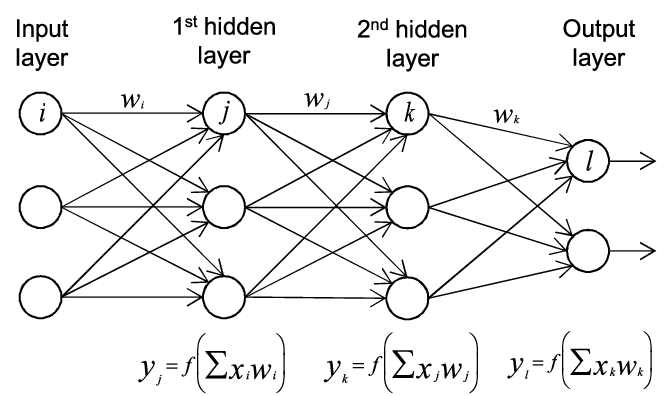
\includegraphics[scale=0.3]{feed-forward_NN.png}
	\caption{NN architecture}
	\label{fig:NN}
\end{figure}


\begin{itemize}
    \gooditem NNs comprise multiple node layers through which data is passed
    \gooditem each layer of nodes trains on a distinct set of features based on the previous layer's output
\end{itemize}

\end{frame}


\begin{frame}{}

For $\theta \in \{ \theta_0, \ldots, \theta_N \}$, introduce the neural network $F^{\theta}: \mathbb{R}^d \rightarrow (0,1)$:
\begin{equation}
F^{\theta}= \psi \circ a_3^{\theta} \circ \phi_{q_2} \circ a_2^{\theta} \circ \phi_{q_1} \circ a_1^{\theta}
\end{equation}
where 
\begin{itemize}
    \gooditem $q_1$ and $q_2$ are the number of nodes in the hidden layers
    \gooditem $a_1^{\theta} : \mathbb{R}^d \rightarrow \mathbb{R}^{q_1}, a_2^{\theta}: \mathbb{R}^{q_1} \rightarrow \mathbb{R}^{q_2}$ are affine functions : $a_i^{\theta}(x)=W_i x + b_i$ 
    \gooditem $\phi_{q_1}: \mathbb{R}^{q_1} \rightarrow \mathbb{R}^{q_1}$ is the ReLU activation function: $\phi_{q_1}(x_i, \ldots, x_{q_i})=(x_i^{+}, \ldots, x_{q_i}^{+})$
    \gooditem $\psi:\mathbb{R} \rightarrow \mathbb{R}$ is the logistic sigmoid function: $\psi(x)=1/(1+ e^{-x})$
\end{itemize}


\medskip
$F^{\theta}$ outputs stopping probabilities $\in (0,1)$ as opposed to stopping decisions $f^{\theta}$ because the gradient-based optimization requires continuous output.

\end{frame}

\begin{frame}{Parameter space}
\begin{itemize}
    \gooditem the parameter space $\theta \in \mathbb{R}^q$ of $F^{\theta}$ is made of $\theta = \{ W_1, W_2, b_1, b_2 \}$, where $W_1 \in \mathbb{R}^{q_1 \times d}, W_2 \in \mathbb{R}^{q_2 \times q_1}, W_3 \in \mathbb{R}^{q_2 \times 1}$ and $b_1 \in \mathbb{R}^{q_1}, b_2 \in \mathbb{R}^{q_2}, b_3 \in \mathbb{R}^{1}$ are the matrices and vectors of the affine functions
    \begin{equation}\label{eq17}
        a^{\theta}_i (x) = W_i x + b_i, \;\;\;\; i =1, 2
    \end{equation}
    \gooditem the dimension of the parameter space is: 
    \begin{equation*}\label{eq18}
        q = 1+q_1+q_2+dq_1+dq_2+q_1 q_2
    \end{equation*}
    for a NN depth of $2$
\end{itemize}
\end{frame}

\begin{frame}{Stochastic Gradient Descent - digression}
at every time step $n = N-1, \ldots, 1$, we have:

\medskip
\begin{itemize}
    \gooditem \textbf{Training dataset:} simulate sample paths $(x^m_n)_{n=1}^N$ for $m=1, \ldots, M$
    \gooditem \textbf{Loss function:} minimize a loss function (e.g. mean squared-error) $C(\theta)$ with respect to $\theta$ and set the model parameters using the training data
    \gooditem \textbf{Gradient:} $\nabla_{\theta}C(\theta^t)$ is computed via backpropagation
    \gooditem \textbf{Update:} the optimal parameters are found by minimizing $C(\theta)$ via a gradient descent algorithm. e.g. with learning rate $\eta$
    \begin{equation}\label{eq19}
    \theta_{t+1} \leftarrow \theta^t - \eta \cdot \nabla_{\theta}C(\theta^t)
    \end{equation}
    This is equivalent to maximizing the reward function

    \gooditem \textbf{Testing dataset:} simulate new sample paths $(y^m_n)_{n=1}^N$ and run the algorithm using the optimized parameters from \ref{eq19},  
\end{itemize}
\end{frame}

\begin{frame}{Reward function $C(\theta)$}
\begin{alertblock}{Objective}

By backward recursion, find the optimal stopping time $\tau^{\ast}$ in \ref{eq1} that maximizes the expected future reward.

\medskip
\begin{itemize}
    \gooditem At $n=N$ we set $f_N \equiv 1$ and the reward is $g(N, X_N)$
    \gooditem At each timestep $n$ we can 
    \begin{itemize}
        \gooditem stop $(f_n(X_n)=1)$ and receive reward of $g(n, X_n)$
        \gooditem continue $(f_n(X_n)=0)$ and then proceed behaving optimally and receive a reward of $g(\tau_{n+1}, X_{\tau_{n+1}})$
        \end{itemize}
        This translates into finding function $f:\mathbb{R}^d \rightarrow \{0,1\}$ that maximizes

        \begin{equation}\label{eq20}
            \mathbb{E}[g(n, X_n)f(X_n) + g(\tau_{n+1}, X_{\tau_{n+1}})(1-f(X_n))]
        \end{equation}
\end{itemize}
\end{alertblock}


\end{frame}


\begin{frame}{}

The stochastic gradient ascent optimization algorithm computes the NN parameters $\theta$ that approximates the objective function:
\begin{equation}\label{eq21}
    \sup_{\theta \in \mathbb{R}^q} \mathbb{E}[g(n, X_n)F^{\theta}(X_n) + g(\tau_{n+1}, X_{\tau_{n+1}})(1-F^{\theta}(X_n))]
\end{equation}

by iteratively maximizing the objective function for $n=N-1, \ldots, 1$ with $F^{\theta_N} \equiv 1$:
\begin{equation}\label{eq22}
    \mathbb{E}[g(n, X_n)F^{\theta_n}(X_n) + g(\tau_{n+1}, X_{\tau_{n+1}})(1-F^{\theta_n}(X_n))]
\end{equation}
which produces a value close to \ref{eq21}

\medskip
Once $\theta_n \in \mathbb{R}^q$ are obtained, $F^{\theta_n}$ is transformed into a stopping decision $f^{\theta_n} \in \mathbb{R}^q \rightarrow \{0,1 \}$

\end{frame}

\begin{frame}{An application}



\end{frame}



%-----------------------------------------------------------------------------------------------------
%% Optimal switching %%
%-----------------------------------------------------------------------------------------------------


\begin{frame}
\frametitle{Optimal switching}
Let the stochastic system that operate in $2$ regimes $\mathbb{I}=\{0,1 \}$.
\begin{itemize}
    \gooditem regimes can be switched at a sequence of stopping times over a finite horizon $[0, \ldots , T]$
    \gooditem there is a payoff rate per unit of time when the system is in mode $i \in \mathbb{I}$ at time $t$ as a mapping $\Psi_i(t, X_t): \Omega \times [0, T] \rightarrow \mathbb{R}$
    \gooditem there is a cost for switching from regime $i$ to $j$ given by the function $\gamma_{i, j} : \Omega \times [0, T] \rightarrow \mathbb{R} $ to cover for the extra costs due to the change of the regime
\end{itemize}


 



\end{frame}


\begin{frame}{Management strategy}
A strategy $\alpha$ for the power plant is a combination of two sequences:
\begin{itemize}
    \gooditem non decreasing sequence of $\mathbb{F}$-stopping times $(\tau_n)_{n \geq 1}$, $n \in \mathbb{N} \backslash \{0\}$, where at $\tau_n$ the production is switched from the current mode $i$ to $j$. Assume: $\tau_0=t$ and $\tau_n \leq \tau_{n+1}$.
    \gooditem a sequence of indicators $(\iota)_{n \geq 1}$, $n \in \mathbb{N} \backslash \{0\}$, $\mathcal{F}_{\tau_n}$- measurable valued in $\mathbb{I}_m$. At time $t=\tau_n$ the system is switched from the current regime $\iota_{n-1}$ to $\iota_{n}$, with $\iota_{0}=i$.
\end{itemize}
\medskip

Denote by $\mathcal{A}_{t, i}$ the set of admissible strategies to switch at time $\tau_n$, $n \geq 1$, from the current regime $\iota_{n-1}$ to $\iota_{n}$. 
\end{frame}

\begin{frame}
\frametitle{Objective function}
For any initial condition $(x, i) \in [0, T] \times \mathbb{I}_m$, and any control $\alpha=(\tau_n, \iota_n)_{n \leq 0} \in \mathcal{A}_{t, i}$. the total expected payoff up to $T$ for such strategy can be expressed as: 
\begin{equation}\label{eq23}
J_i(x, \alpha) = \mathbb{E} \Big[ \sum_{s=t}^{T-1} \Psi(X_t^{x, i}, I_t^i) + \Gamma - \sum_{n \leq 1}\gamma_{\iota_{n-1}, \iota_n} \mathbf{1}_{ \{ \tau_n < T \} }  | \mathcal{F}_n   \Big]
\end{equation}

The objective is to maximize this expected total profit for all strategies $\alpha$. For this purpose, we set the value function:
\begin{equation}\label{eq24}
V_i(x)=\sup_{\alpha \in \mathcal{A}} J_i(x, \alpha) \;\;\;\;\;\;\;\;\; \forall \alpha \in \mathcal{A}_{t, i} \,\, \mathbb{P}\; a.s. 
\end{equation}
\end{frame}


\begin{frame}{Proposed approach}
Following the approach given by \cite{becker2019deep}, we want to provide a solution to the optimal switching problem in \ref{eq24}. This requires
\begin{enumerate}
    \gooditem express stopping times as a series of stopping decisions
    \gooditem approximate these $0-1$ stopping decisions using a neural network
\end{enumerate}
\end{frame}

\begin{frame}{}
\begin{equation}
\check{Y}_{N}^i = \Gamma \\
\check{Y}_{n}^i = \Psi_i(n) + \max_{j \in \{0, 1 \}} 
\{- \gamma_{i, j}(n) + e^{-\rho h} \check{Y}_{n+1}^j   \} \;\;\;\;\;\;\;\;\;\; \text{for } n=N-1, \ldots, 0
\end{equation}
\end{frame}

\begin{frame}{An application}
some elements of the system:
\begin{itemize}
    \gooditem payoff function for the call option used is of the form $( \max_{i \in \{ 1, \ldots , d \}} X_t^i - K) ^{+}$, where $K$ is the strike price at any point in the time grid $0 = t_0 < t_1 < \ldots < t_N = T$
    \gooditem the system also outputs a final reward for being in mode $i \in \mathbb{I}$ at time $T$ given by $\Gamma_i$
\end{itemize}
\end{frame}

%----------------------------------------------------------------------------
\begin{frame}{Training performance}

\begin{figure}[H] 
\centering
\begin{subfigure}{.5\textwidth}
  \centering
  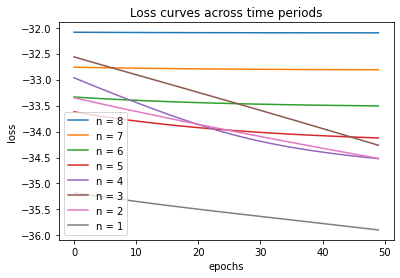
\includegraphics[width=.25\linewidth]{loss_curves_optStopping.png}
  \caption{Optimal Stopping}
  \label{fig:sub1}
\end{subfigure}%
\begin{subfigure}{.5\textwidth}
  \centering
  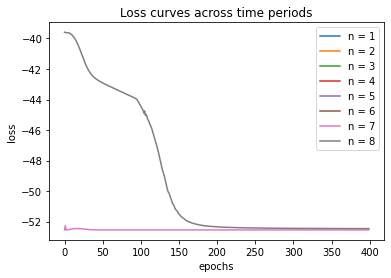
\includegraphics[width=.25\linewidth]{loss_curves_optSwitching.png}
  \caption{Optimal Switching}
  \label{fig:sub2}
\end{subfigure}
\caption{Loss curves (train) for 8 time steps}
\label{fig:test}
\end{figure}


\begin{itemize}
    \gooditem payoff function for the call option used is of the form $( \max_{i \in \{ 1, \ldots , d \}} X_t^i - K) ^{+}$, where $K$ is the strike price at any point in the time grid $0 = t_0 < t_1 < \ldots < t_N = T$
    \gooditem the system also outputs a final reward for being in mode $i \in \mathbb{I}$ at time $T$ given by $\Gamma_i$
\end{itemize}
\end{frame}

%-----------------------------------------------------------------------------------------------------
%% Least Square Policy Iteration %%
%-----------------------------------------------------------------------------------------------------
\begin{frame}{}

\cite{longstaff2001valuing} approximate continuation value for the decision to stop or to continue
most used method in the financial industry
If $\mathbb{E}[U_{t_n+1}| \mathcal{F}_{t_n}]$ is known, an optimal stopping time policy can be synthesized explicitly by stopping if and only if $Z_{t_n} \geq  \mathbb{E}[U_{t_n+1}| \mathcal{F}_{t_n}]$. The algorithm proposed approximates the continuation value as:  
\begin{equation}
    c_{\theta}
\end{equation}
convergence guarantees
do not easily scale to high
dimensional problems since the number of basis functions usually grows polynomially or
even exponentially (Longstaff and Schwartz, 2001, Section 2.2) in the number of stocks. One
direction of research to overcome this problem is to apply dimension reduction techniques \citep{bayer2021pricing}
\end{frame}


\begin{frame}
\frametitle{Least Square Policy Iteration}
A policy $\pi$ is a behavior function that maps states to actions:
\begin{equation}
a = \pi(s)
\end{equation}

If we consider a full episode (one of our complete trajectories) that starts at time t=0 and terminates at time t=T, then we define the return R₀ from the starting state as:

\begin{equation}
R_0 = \sum_{t=0}^T \gamma^t r_t
\end{equation}
Where $r_t$ is the reward at time $=t$, and $\gamma$ is a discount factor in the range $[0,1]$, which allows us to adjust the time horizon, and ensure the return over long episodes remains finite. 

As the transition from state $s \rightarrow s^{\prime}$ is generally probabilistic (starting multiple episodes from the same state will generally result in different returns), we take the expectation value of return over all allowed trajectories. By doing so, we can define the expected return, called the state-value function $V_{\pi}$ which describes the expected return starting from state $s$ and then following policy $\pi$:

\begin{equation}
V_{\pi} =  \mathbb{E}[R_t | s_t = s_t] 
\end{equation}
where $R_t$ is the return of a single, specific full episode starting at time $t$. The expectation operator $\mathbb{E}[\cdot]$ averages over all possible individual episodes/trajectories starting from initial state $s$ and following policy $\pi$. 

A closely related quantity is the action-value function $Q_{\pi}$ which describes the expected return starting in state $s$, taking action $a$, and thereafter following policy $\pi$:

\begin{equation}
Q_{\pi}(s,a) =  \mathbb{E}_{a_t \sim \pi; s_t \sim \mathcal{P}}[R_0 | s_0 = s, a_0 = a] 
\end{equation}

In most scenarios, the underlying MDP model is not fully available. Typically, the state space, the action space, and the discount factor are available, whereas the transition model and the reward function are not known in advance. It is still desirable to be able to evaluate, or, even better, find good decision policies. Here we rely on information that comes from interaction between the decision maker and the process itself, hence tuples known as samples: 
\begin{equation}
(s, a, r, s^{\prime})
\end{equation}
Samples are collected from actual (sequential) episodes of interaction with the processand the algorithm learns decision policies from such samples.

\end{frame}

\begin{frame}
In our algorithm, we approximate the action-value function $Q_{\pi}(s, a)$ by a linear architecture and its actual representation consists of a compact
description of the basis functions and a set of parameters

$Q_{\pi}$ values are approximated by a linear parametric combination of
$k$ basis functions (features):
\begin{equation}
\hat{Q}_{\pi}(s,a; w) = \sum_{j=1}^k \phi_j (s,a) w_j
\end{equation}

where the $w_j$’s are the parameters. The basis functions $\phi_j (s,a)$ are fixed, but arbitrary and, in general, non-linear, functions of $s$ and $a$. We require that the basis functions $\phi_j$ are linearly independent to ensure that there are no redundant parameters and that the matrices involved in the computations are full rank. Typical linear approximation architectures are polynomials of any degree (each basis function is a polynomial term) and
radial basis functions (each basis function is a Gaussian with fixed mean and variance).

Define $\phi(s,a)$ to be the column vector of size $k$ where each entry $j$ is the corresponding basis function $\phi_j$ computed at $(s,a)$:
\begin{align}
\phi(s,a) =
 \begin{pmatrix}
  \phi_1(s,a) \\
  \ldots \\
  \phi_k(s,a) 
 \end{pmatrix}
\end{align}

Now, $\hat{Q}_{\pi}$ can be expressed compactly as $\hat{Q}^{\pi} = \mathbf{\Phi}w^{\pi}$, where $w^{\pi}$ is a column vector of length $k$ with all parameters and $\mathbf{\Phi}$ is a $(|\mathcal{S}||\mathcal{A}| × k)$ matrix, where each row contains the value of all basis functions for a certain pair $(s,a)$ and each column the value of a certain basis function for all pairs $(s,a)$.
\end{frame}

\begin{frame}
\frametitle{Update rule}
Consider the problem of learning the (weighted) least-squares fixed-point approximation $\hat{Q}_{\pi}$ to the state-action value function $Q_{\pi}$ of a fixed policy $\pi$ from samples. Assuming that there are $k$ linearly independent basis functions in the linear architecture, this problem is
equivalent to learning the parameters $w^{\pi}$ of $\hat{Q}_{\pi} = \mathbf{\Phi}w^{\pi}$. The exact values for $w^{\pi}$ can be computed from the model by solving the $(k × k)$ linear system:

\begin{equation}
\mathbf{A} w^{\pi}= b,
\end{equation}
where
\begin{equation}
\mathbf{A} = \mathbf{\Phi}^\intercal \Delta_{\mu} (\mathbf{\Phi} − \gamma \mathbf{P} \mathbf{\Pi}_{\pi} \mathbf{\Phi})\;\;\;\; \text{and} \;\;\;\; b =\mathbf{\Phi}^\intercal \Delta_{\mu} \mathcal{R} ,
\end{equation}
and $\mu$ is a probability distribution over $S × A)$ that defines the weights of the projection.

For the learning problem, $\mathbf{A}$ and $b$ cannot be determined a priori, either because the matrix $\mathbf{P}$ and the vector $\mathcal{R}$ are unknown, or because they are so large that they cannot be used in any practical computation. However, $\mathbf{A}$ and $b$ can be learned using samples; the
learned linear system can then be solved to yield the learned parameters we
$\pi$ which, in turn, determine the learned value function.

So, given any finite set of $L$ samples:
\begin{equation}
D = \Big\{(s_i, a_i, r_i, s^{\prime}_i), i =1, \ldots, L     \Big\}
\end{equation}

then we can compute $\mathbf{A}$ and b as:

\begin{equation}
\tilde{\mathbf{A}} = \frac{1}{L} \sum_{i=1}^L \Bigg[\phi(s_i, a_i) \Big(\phi(s_i, a_i) - \gamma \phi(s_i^{\prime}, \pi(s_i^{\prime} )   \Big)^{\intercal} \Bigg]\\
\tilde{b} = \frac{1}{L} \sum_{i=1}^L  \Bigg[\phi(s_i, a_i) r_i \Bigg]
\end{equation}
assuming that the distribution $\mu_{D}$ of the samples in $D$ over $(\mathcal{S} \times \mathcal{A})$ matches the desired distribution. Clearly, the learned approximation is biased by the distribution $\mu_{D}$ of samples. In general, the distribution $\mu_{D}$ might be different from the desired distribution $\mu$. This problem would be resolved trivially when a generative model is available, since samples can be drawn so that $\mu_{D} = \mu$.


Given that a single sample contributes to $\tilde{\mathbf{A}}$ and $\tilde{b}$ additively, it is easy to construct an incremental update rule for these. Let $\tilde{\mathbf{A}}^{(t)}$ and $\tilde{b}^{(t)}$ be the current learned estimates of $\mathbf{A}$ and $b$ for a fixed policy $\pi$, assuming that initially $\tilde{\mathbf{A}}^{(0)} = 0$ and $\tilde{b}^{(0)} = 0$. A new sample
$(s_t, a_t, r_t,s^{\prime}_t)$ contributes to the approximation according to the following update equations:

\begin{equation}
\tilde{\mathbf{A}}^{t+1} = \tilde{\mathbf{A}}^{t} + \phi(s_i, a_i) \Big(\phi(s_i, a_i) - \gamma \phi(s_i^{\prime}, \pi(s_i^{\prime} )   \Big)^{\intercal}\\
\tilde{b}^{t+1} = \tilde{b}^{\prime} + \phi(s_i, a_i) r_i 
\end{equation}

From these results we can then proceed to learn the weighted least-squares
fixed-point approximation of the state-action value function of a fixed policy $\pi$ from samples in a batch or in an incremental way.  
\end{frame}

\appendix
\section{More}
\begin{frame}[label=supplemental]
Supplemental content.
Back to \hyperlink{main}{\beamerbutton{main}}.
\end{frame}



\begin{frame}{References}

\bibliography{references_main}
\bibliographystyle{agsm}
  
\end{frame}  
  
\end{document}